%------------------------------------------------------------------------------------
%	CHAPTER 1
%------------------------------------------------------------------------------------
\chapterimage{headMontagem.png}
\chapter{Entendimento Geral}

\begin{remark}
"A tecnologia é uma faísca criativa que ilumina as mentes e transforma a maneira como vemos e interagimos com o mundo." (Steve Jobs) 
\end{remark}

\section{Do que trata esse livro?}\index{Entendimento Geral}
\textbf{Apache Spark} (a palavra pode ser traduzida para "centelha" ou faísca") pois seu objetivo é dar velocidade e eficiência ao processamento de dados. Assim como uma centelha energética, seu objetivo é de uma maior produtividade e desempenho em projetos de análise e processamento de informações. Com sua capacidade de processar grandes volumes de dados de forma distribuída, Apache Spark acelera o ritmo das descobertas, permite que empresas se destaquem na era da transformação digital. Com essa poderosa ferramenta, é possível acender a faísca da inovação e alcançar resultados surpreendentes, explorando todo o potencial dos dados para impulsionar o crescimento e a competitividade.

Apache Spark (para abreviar pretendo chamá-lo somente de Spark) possui uma poderosa e veloz arquitetura para processamento em tempo real, pois sua principal vantagem reside na capacidade de realizar cálculos em memória, e isso acelera significativamente a análise de dados. Surgindo como resposta à limitação do \textbf{Apache Hadoop MapReduce}, que se restringia a processamentos em lote, Spark preencheu a lacuna ao introduzir o processamento de \textit{stream} (fila de dados) em tempo real. Tornou-se inclusive um componente essencial desse ambiente.

Possui uma arquitetura distribuída, isso significa que pode ser escalado horizontalmente em vários nós de computação, e assim possibilitar o processamento eficiente para grandes volumes de dados. Adequado para lidar com conjuntos de dados que varia de terabytes ou até petabytes.

\section{O que é Apache Spark?}\index{Entendimento Geral}
A arquitetura do Spark foi projetada para superar as limitações do \textbf{Hadoop MapReduce} e oferecer um ambiente de processamento de dados mais rápido e flexível. Ao contrário do \textbf{Hadoop MapReduce}, que requer a leitura e escrita repetida de dados no disco, Spark utiliza uma estrutura de processamento em memória, isso permite operações mais ágeis e eficientes. Essa abordagem executa análises mais complexas em tempo real, acelera o tempo de resposta e abre novas possibilidades de aplicação.

Spark é uma plataforma com processamento de dados que possui seu próprio gerenciador de cluster, isso permite hospedar aplicativos diretamente nele. Além disso, faz uso do \textbf{Hadoop}, aproveitando o sistema de arquivo distribuído \textbf{HDFS} (\textit{Hadoop Distributed File System}) para armazenamento e o \textbf{YARN} para executar os aplicativos distribuídos.

Originalmente foi desenvolvido para usar a linguagem de programação \textbf{Scala}, porém expandiu suas funcionalidades para oferecer suporte a \textbf{Python} por meio de uma ferramenta chamada \textbf{PySpark}. Com essa ferramenta, os usuários podem trabalhar com \textbf{RDD} (\textit{Resilient Distributed Dataset}), que é uma abstração de dados resiliente distribuída, na linguagem de programação Python. E isso amplia as possibilidades de desenvolvimento e análise de dados, permite aos programadores utilizar a linguagem de sua preferência para aproveitar o poder e a flexibilidade do Spark.

\section{Montagem do Ambiente}\index{Entendimento Geral}
Atualmente, presenciamos uma revolução no campo da Ciência de Dados, com constantes avanços e atualizações nas ferramentas utilizadas nessa área. No entanto, é importante destacar que essas atualizações rápidas podem trazer consigo problemas que afetam diretamente o sistema operacional. Surge então a pergunta: Como podemos nos manter atualizados e seguros ao mesmo tempo? A resposta que se destaca como a mais coerente é a utilização da técnica de conteinerização para resolver esse problema.

A conteinerização é uma abordagem que permite empacotar um aplicativo e todas as suas dependências em um contêiner isolado. Com isso, é possível garantir que as atualizações e modificações necessárias sejam feitas dentro do contêiner, sem afetar o nosso sistema operacional. Essa abordagem proporciona uma camada adicional de segurança, uma vez que os contêineres são isolados uns dos outros e do ambiente de hospedagem.

Ao utilizar a conteinerização, é possível manter-se atualizado com as últimas versões das ferramentas, aproveitando os benefícios das atualizações sem correr o risco de afetar a estabilidade do sistema operacional. Além disso, os contêineres podem ser facilmente replicados e distribuídos em diferentes ambientes, garantindo consistência e portabilidade.

Uma das ferramentas populares para conteinerização é o \textbf{Docker}, que permite criar, implantar e gerenciar contêineres de forma eficiente. Com o Docker, é possível construir imagens personalizadas contendo as bibliotecas e dependências necessárias para suas aplicações de Data Science, facilitando a reprodução e compartilhamento do ambiente de desenvolvimento.
\begin{figure}[H]
 \centering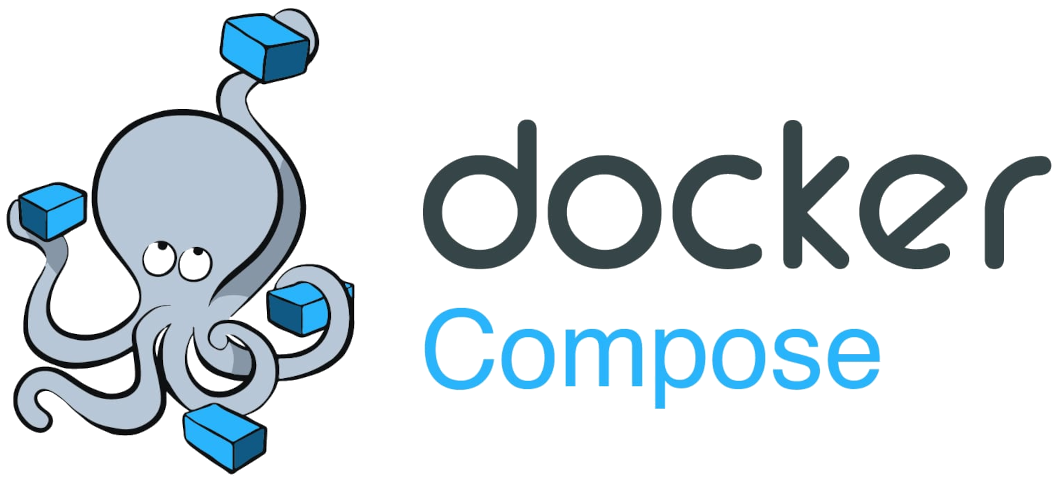
\includegraphics[scale=1.0]{cap01/DockerCompose}
 \caption{Docker Compose para Gerenciamento de Contêineres}
\end{figure}

\textbf{Docker Compose} é uma ferramenta que permite definir e gerenciar múltiplos contêineres com uma simples configuração de arquivos \textbf{YAML}. Projetado para simplificar o processo de criação e execução de aplicativos compostos por vários contêineres Docker interagindo entre si. Podemos simplesmente descrever a configuração dos aplicativos, incluindo quais contêineres serão usados, as redes e volumes necessários, bem como as variáveis de ambiente e outras configurações específicas.

Docker Compose oferece uma série de benefícios. Simplifica o processo para a implantação de aplicativos compostos por múltiplos contêineres, pois tudo é definido em um único arquivo. Isso torna o compartilhamento e a colaboração mais fáceis, pois toda a configuração está documentada em um local central. Além disso, facilita a escalabilidade do aplicativo. Podemos especificar número de réplicas para determinado serviço e o Docker Compose se encarrega de criar e gerenciar os contêineres necessários para atender a essa demanda.

Porquê vários contêineres? Pelo simples fato que precisamos de um editor (no caso o escolhido foi o JupyterLab), um \textbf{Spark Master} e alguns \textbf{Spark Workers} além obviamente de um \textbf{HDFS} para realizar as transações. Basicamente funciona assim:
\begin{itemize} \vspace{-1em}
  \item No JupyterLab podemos dar o comando para realizar qualquer atividade.
  \item Essa é interceptada pelo \textbf{Spark Master} que a repassará para os \textbf{Spark Workers} disponíveis que se encarregarão de sua execução.
\end{itemize}

Graficamente seria essa imagem:
\begin{figure}[H]
	\centering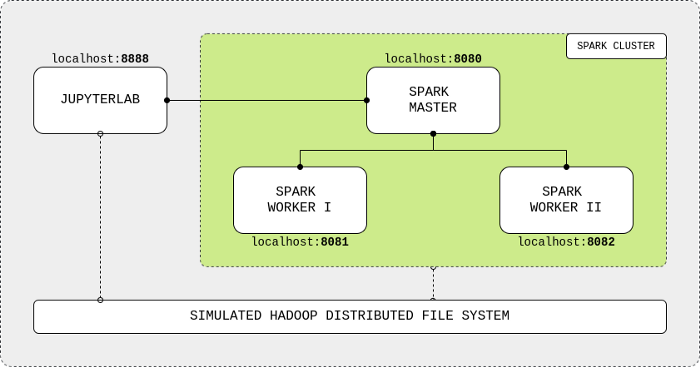
\includegraphics[scale=0.45]{cap01/Arquitetura}
	\caption{Arquitetura do Ambiente}
\end{figure}

A ideia original veio do \textbf{André Perez} que consiste na montagem de imagens Docker e a criação de um ambiente através do Docker Compose. O único detalhe que adicionei foi transpor de forma mais fácil para o iniciante. Primeiro devemos criar uma pasta para comportar os arquivos necessários que conterão os códigos para a criação das dos contêineres necessários e suas respectivas imagens.

\textbf{Parte 1} - Criar um arquivo chamado \textbf{cluster-base.Dockerfile} (\textbf{ATENÇÃO}: Respeite as letras maiúsculas e minúsculas dos nomes e de seu conteúdo, tudo aqui é \textit{case-sensitive}) que servirá como camada base com o Sistema Operacional e o Python 3, através da seguinte codificação:
\begin{lstlisting}[]
FROM openjdk:8-jre-slim

RUN mkdir -p /opt/workspace && \
    apt-get update -y && \
    apt-get install -y python3 && \
    ln -s /usr/bin/python3 /usr/bin/python && \
    rm -rf /var/lib/apt/lists/*

ENV SHARED_WORKSPACE=/opt/workspace
VOLUME /opt/workspace
CMD ["bash"]
\end{lstlisting}

Para sua execução digite o seguinte comando: \\
{\ttfamily\$ docker build -f cluster-base.Dockerfile -t cluster-base .}

\textbf{Parte 2} - Criar um arquivo chamado \textbf{spark-base.Dockerfile} que é a nossa camada Spark, através da seguinte codificação:
\begin{lstlisting}[]
FROM cluster-base

RUN apt-get update -y && \
    apt-get install -y curl && \
    curl https://archive.apache.org/dist/spark/spark-3.4.1/spark-3.4.1-bin-hadoop3.tgz -o spark.tgz && \
    tar -xf spark.tgz && \
    mv spark-3.4.1-bin-hadoop3 /usr/bin/ && \
    mkdir /usr/bin/spark-3.4.1-bin-hadoop3/logs && \
    rm spark.tgz

ENV SPARK_HOME /usr/bin/spark-3.4.1-bin-hadoop3
ENV SPARK_MASTER_HOST spark-master
ENV SPARK_MASTER_PORT 7077
ENV PYSPARK_PYTHON python3
WORKDIR ${SPARK_HOME}
\end{lstlisting}

Para sua execução digite o seguinte comando: \\
{\ttfamily\$ docker build -f spark-base.Dockerfile -t spark-base .}
 
\textbf{Parte 3} - Criar um arquivo chamado \textbf{spark-master.Dockerfile} que é o nosso Spark Master, através da seguinte codificação:
\begin{lstlisting}[]
FROM spark-base
EXPOSE 8080 ${SPARK_MASTER_PORT}
CMD bin/spark-class org.apache.spark.deploy.master.Master >> logs/spark-master.out
\end{lstlisting}

Para sua execução digite o seguinte comando: \\
{\ttfamily\$ docker build -f spark-master.Dockerfile -t spark-master .} 
 
\textbf{Parte 4} - Criar um arquivo chamado \textbf{spark-worker.Dockerfile} que é o nosso Spark Worker, através da seguinte codificação:
\begin{lstlisting}[]
FROM spark-base
EXPOSE 8081
CMD bin/spark-class org.apache.spark.deploy.worker.Worker spark://${SPARK_MASTER_HOST}:${SPARK_MASTER_PORT} >> logs/spark-worker.out
\end{lstlisting}

Para sua execução digite o seguinte comando: \\
{\ttfamily\$ docker build -f spark-worker.Dockerfile -t spark-worker .} 
 
\textbf{Parte 5} - Criar um arquivo chamado \textbf{jupyterlab.Dockerfile} que é o nosso editor, através da seguinte codificação:
\begin{lstlisting}[]
FROM cluster-base

RUN apt-get update -y
RUN apt-get install -y python3-pip
RUN pip3 install pyspark==3.4.1
RUN pip3 install jupyterlab

EXPOSE 8888
WORKDIR ${SHARED_WORKSPACE}
CMD jupyter lab --ip=0.0.0.0 --port=8888 --no-browser --allow-root --NotebookApp.token=spark
\end{lstlisting}

Para sua execução digite o seguinte comando: \\
{\ttfamily\$ docker build -f jupyterlab.Dockerfile -t jupyterlab .} 

Após essa etapa, temos cinco imagens que possuem uma dependência interligada, representada graficamente da seguinte forma:
\begin{figure}[H]
	\centering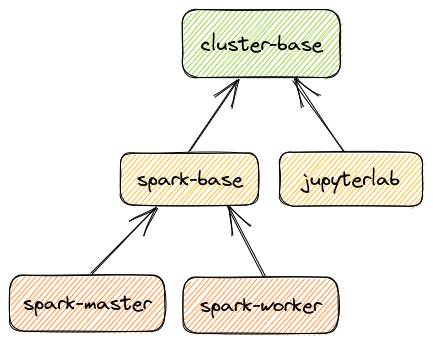
\includegraphics[scale=0.45]{cap01/ImagensDocker}
	\caption{Dependência das imagens geradas}
\end{figure}

Basicamente, precisamos de três delas: \textbf{jupyterlab} (editor de códigos), \textbf{spark-master} e \textbf{spark-worker}. No entanto, é mais conveniente criar uma imagem base chamada \textbf{cluster-base}, que contém as informações do sistema operacional utilizado. Além disso, uma segunda imagem fundamental para o Spark é obtida pela \textbf{spark-base}, que instala uma instância do Spark sobre o Hadoop,

\begin{note}[Porquê no Linux?] 
	Sinto se você é fã do Windows ou Mac, nada contra esses sistemas operacionais, porém preciso de um ambiente robusto e que o Docker seja nativo, se conseguir transpor todos os comandos mostrados aqui no shell para esses ambientes não terá muitos problemas. Aqui utilizei o \textbf{Linux Ubuntu}.
\end{note}

O último passo é o mais simples de todos e aí que entra o \textbf{docker compose}, precisamos a partir dessas imagens subir um contêiner da imagem do \textbf{jupyterlab}, mais um com a imagem do \textbf{spark-master} e ao menos dois (pode futuramente adicionar novos se assim desejar) com \textbf{spark-worker} e ligá-las na rede além de passar alguns passos para sua criação. Isso tudo será feito através de um arquivo chamado \textbf{docker-compose.yml} que possui o seguinte conteúdo:
\begin{lstlisting}[]
version: "3.6"
services:
  jupyterlab:
    image: jupyterlab
    container_name: jupyterlab
    ports:
      - 8888:8888
    volumes:
      - /home/fernando/meu-spark:/opt/workspace
  spark-master:
    image: spark-master
    container_name: spark-master
    ports:
      - 8080:8080
      - 7077:7077
    volumes:
      - /home/fernando/meu-spark:/opt/workspace
  spark-worker-1:
    image: spark-worker
    container_name: spark-worker-1
    environment:
      - SPARK_WORKER_CORES=1
      - SPARK_WORKER_MEMORY=512m
    ports:
      - 8081:8081
    volumes:
      - /home/fernando/meu-spark:/opt/workspace
    depends_on:
      - spark-master
  spark-worker-2:
    image: spark-worker
    container_name: spark-worker-2
    environment:
      - SPARK_WORKER_CORES=1
      - SPARK_WORKER_MEMORY=512m
    ports:
      - 8082:8081
    volumes:
      - /home/fernando/meu-spark:/opt/workspace
    depends_on:
      - spark-master
\end{lstlisting}

A pasta "/home/fernando/meu-spark" se refere a um caminho na minha máquina, modifique-o conforme seu sistema e endereçamento.

Para cada \textbf{spark-worker} estabelecemos memória de 512 Mb, isso será necessário para que tenham boa performance, mas como citado aumente o número conforme a necessidade. O primeiro usará a porta 8081 e segundo a 8082. O \textbf{spark-marter} responde nas portas 8080 e 7077.

Quanto a rede, para rodarmos os contêineres iremos necessitar de uma rede, o nome dessa será a pasta que se encontra este arquivo YAML, sendo assim, vamos supor que a pasta se chama "pyspark-docker", então o seguinte comando deve ser executado: \\
{\ttfamily\$ docker network create pyspark-docker\_default}

Para criar os nossos contêineres: \\
{\ttfamily\$ docker-compose create}

Para executá-los: \\
{\ttfamily\$ docker-compose start}

Como resposta deve ter recebido: \\
{\ttfamily Starting jupyterlab     ... done \\
Starting spark-master   ... done \\
Starting spark-worker-1 ... done \\
Starting spark-worker-2 ... done}

Se digitar o comando: \\
{\ttfamily\$ docker ps}

Verá que os quatro contêineres estão ativos em suas respectivas portas, para pará-los: \\
{\ttfamily\$ docker-compose stop}

Lembre-se que sempre estes comandos devem ser dados nesta pasta específica aonde está o arquivo \textbf{docker-compose.ylm}.

\begin{note}[Deu erro!] 
	Provavelmente o nome da sua rede está errado, verifique se o erro é esse aqui: ERROR: for jupyterlab  Cannot start service jupyterlab: network "Nome da Rede" not found.
\end{note}
 
Com os contêineres ativos, abrir o navegador no endereço \url{http://localhost:8888} e obtemos o seguinte resultado:
\begin{figure}[H]
	\centering\includegraphics[scale=0.4]{cap01/paginaSenha}
	\caption{Jupyter solicitando o Token}
\end{figure}

A senha do token está definida no arquivo de criação da imagem do JupyterLab como "spark", após informá-la o JupyterLab pronto para trabalharmos:
\begin{figure}[H]
	\centering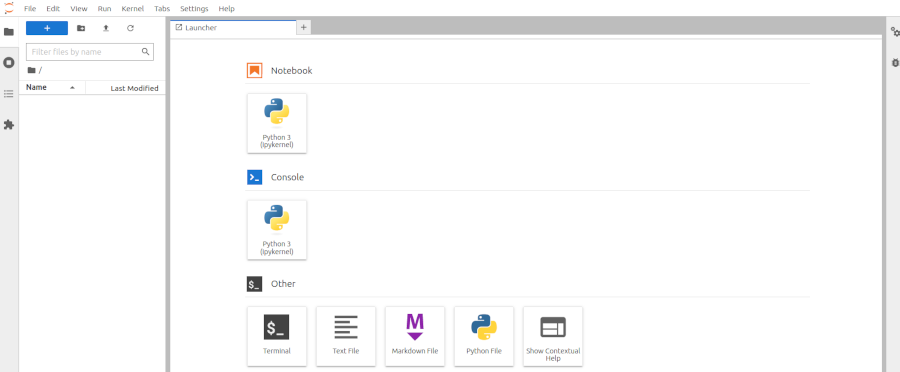
\includegraphics[scale=0.5]{cap01/JupyterLab}
	\caption{Jupyter Lab pronto}
\end{figure}

Verificar qual a versão do Python que está a nossa disposição, crie um Notebook e na primeira célula digite:
\begin{lstlisting}[]
!python --version
\end{lstlisting}

Ao executarmos esta, é mostrada a versão 3.9.2. Agora em outra aba do navegador acesse o endereço \url{http://localhost:8080}, e temos:
\begin{figure}[H]
	\centering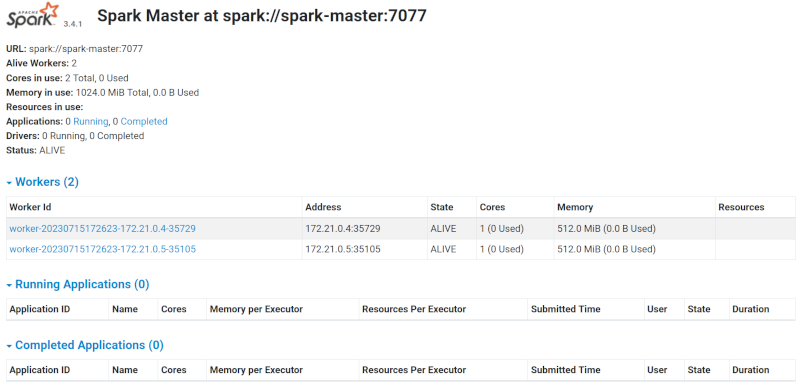
\includegraphics[scale=0.6]{cap01/SparkMaster}
	\caption{Spark Master pronto}
\end{figure}

Isso indica que nosso Spark Master está pronto e possui 2 Spark Workers a disposição. 
Além de suas capacidades em tempo real, Spark também é responsável pelo processamento em lote, assim obtemos uma solução abrangente e flexível. Rapidamente tornou-se a escolha popular para empresas que buscam lidar tanto com cargas de trabalho em tempo real quanto com análises em grande escala. Outro aspecto notável é o suporte e execução de consultas complexas e a aplicação de algoritmos iterativos em larga escala, o que é fundamental para tarefas como aprendizado de máquina e mineração de dados. Com essa funcionalidade, esta é uma ferramenta versátil para uma ampla gama de aplicações que exigem o processamento de dados.

Como dito anteriormente uma das principais motivações para a criação do Spark como substituto do \textbf{Hadoop MapReduce} foi justamente atender às demandas crescentes por velocidade e flexibilidade no processamento de dados. Spark introduziu o conceito de Resilient Distributed Datasets (RDDs), que são estruturas de dados imutáveis e distribuídas, armazenadas em memória e que podem ser processadas de forma paralela. Essa abordagem inovadora permite que o Spark otimize a execução de operações complexas, como transformações e ações, reduzindo a latência e aumentando a eficiência geral do processamento de dados. Veremos isso no próximo capítulo.	

\begin{note}[Não sabe nem por onde começar com o Docker?] 
	Não se desespere, baixe um paper sobre o Docker gratuitamente na minha página no Academia.edu (\url{https://iesbpreve.academia.edu/FernandoAnselmo}).
\end{note}
\clearpage